\documentclass[a4paper,12pt]{article}

% Any percent sign marks a comment to the end of the line

% Every latex document starts with a documentclass declaration like this
% The option dvips allows for graphics, 12pt is the font size, and article
%   is the style

\usepackage[pdftex]{graphicx}
%\usepackage{url}
\usepackage{hyperref}
% These are additional packages for "pdflatex", graphics, and to include
% hyperlinks inside a document.
\usepackage{lettrine}
\setlength{\oddsidemargin}{0.25in}
%\setlength{\textwidth}{6.5in}
\setlength{\topmargin}{0in}
%\setlength{\textheight}{8.5in}

% These force using more of the margins that is the default style
\usepackage{times}
\usepackage{mathptmx}
\usepackage{color}
\usepackage{amssymb}
\usepackage{amsmath}
\begin{document}

% Everything after this becomes content
% Replace the text between curly brackets with your own

\title{SCORE 2018 Project Proposal\\Epic-Monopoly}
\author{\small Ziqiang Li 11510352@mail.sustc.edu.cn\\
\small Yulian Mao 11510086@mail.sustc.edu.cn\\
\small Xizi Ni 11510602@mail.sustc.edu.cn\\
\small Yilin Zheng 11510506@mail.sustc.edu.cn\\
\small Chenyu Zhou 11510374@mail.sustc.edu.cn}
\date{Oct. 2017}

% You can leave out "date" and it will be added automatically for today
% You can change the "\today" date to any text you like


\maketitle

% This command causes the title to be created in the document

\section{Abstract}
\lettrine[lines=2,loversize=0.35,lraise=0.07,findent=3pt,nindent=2pt]{I}{}n this project, we concentrate on developing a new web based monopoly game mechanism which called Epic-Monopoly. There are many new and interesting element evolved in this game. Firstly, economy factor, which can be seen as GDP or relative index, is added into the Epic-Monopoly to make the game closed to reality. The price of the properties (e.g. house, station etc.), the tax and the punishment intensity of the chance card are under the influence of the economy factor. Besides, the difficulty of the Epic-Monopoly also can be decided by the fluctuation of the economy factor. Secondly, in order to add more interesting element as well as balance the game, we use dynamic map in Epic-Monopoly. The player who is falling behind may regain hope with the period changing map. At last, in the reality there are many cooperation between many entrepreneurs, considering the cooperation among the player, the Epic-Monopoly include alliance and countries in to the game, those elements can be also seen as loyalty program. The tax and warfare are decided by those two elements. Despise of those important and creative new silver point, there are some other modification, such as the enterprisers mid entering rules and so on. The details are introduced in the following sections.
\section{Background}
\lettrine[lines=2,loversize=0.35,lraise=0.07,findent=3pt,nindent=2pt]{M}{}r.Wang, Mr.Li, Mr.Son and Mr.Trump, who are enterprisers from China, Japan and America, they want to play a game to decide who is the smartest in business. They play a novel monopoly game, called Epic-Monopoly, which involves more uncertainty with more variables and inexact parameters. Besides, enterprisers are allowed to join in mid. They choose hard mode since they are willing to show confidence and make competitors more difficult to win. Mr.Wang chooses to buy more properties as soon as possible for larger probability that opponents step into his properties which makes his packet more money. Mr.Trump chooses to buy expensive properties and build more rooms for luxury rental which seeks large amount for single charge. Mr.Son invests steadily. And for Mr.Li, he chooses to owning both utilities. As game is processing, Mr.Ma joins in. There are large volatility under hard difficulty. Mr.Trump spends too much money to upgrade the properties which leads to cash shortage, and more worse, he steps into the opponents' property. Since mortgage money cannot pay off his debt after mortgaging all his properties, Mr.Trump finally ends with bankruptcy. Mr.Ma have large amount of cash, so, he auctions into Mr.Trump's properties from the bank at a relatively lower price and takes the leading position soon. In that case, other enterprisers come to realize that they need to unit together for their own benefits. So, they agree to form an alliance in order to protect mutual interests for beating Mr.Ma. The game is getting more and more interesting and much contested.
\section{Current Problems}
	\lettrine[lines=2,loversize=0.35,lraise=0.07,findent=3pt,nindent=2pt]{F}{}irst, the original Monopoly was published in 1935 according to Wikipedia. At that time, due to the technology drawback, it is difficult for game designer to design a dynamic game. Because of previous problem, the original Monopoly is contradicting to real-life economy in some perspective. The value of properties is static which is impossible in real world. Therefore, origin Monopoly must be dynamize.
	
	Second, there are not loyalty program in Monopoly. Rent of real estate stays still in regard of how many times a player paid for the rent. In reality, there are some reward for the renter for paying many times.
	
	Also, the sequence of map cannot change in Monopoly, which must responsible for the loss of many players. If a player buys all the real estate for continues two color blocks, it will have much more chance to win this game. On the other words, the rest of players will lose the fate of winning the game.
	
	Besides, because of lack of rewarding for cooperation, players seldom cooperate with each other. In Monopoly, players always play alone, complete with the rest of players. While on reality, enterprisers always cooperate with each other for the profit.
\section{Solution \& Silver Bullet}
\lettrine[lines=2,loversize=0.35,lraise=0.07,findent=3pt,nindent=2pt]{T}{}here are some solutions for the current problem, but the rules may change during developing process. For the updated information and detail, please see our web page: \href{https://epicmonopoly.github.io}{\color{blue}{EpicMonopoly}}
\begin{itemize}
	\item Economy Factor
	
	Analogy from GDP or some relative economic index, Economy Factor(EF) is considered in the Epic-Monopoly. EF act as a “global ruler”, is in charge of the change of the price of properties, tax and value of other object. Also, introducing EF in to Epic-Monopoly can also balance the game dynamically.
	
	For a specific period, EF will change between a certain range, and it will have influence on the rent, pricing of the house, etc. Because of its characteristic, the average value of all property is same. It is seldom for a property devalue every period, which is unfortunate for the owner of this property.
	
	\item Dynamic Map
	The sequence of spot in the Epic-Monopoly will change in a specific period, to repick the fate of players who falling behind. To unified the map, the change of color blocks, stations and utilities will be control by some rules.
	
	\item Country \& Alliance
	
	For the cooperation problem, countries and alliances are introduced to the Epic-Monopoly. Every player will assign to one countries and corresponding alliances. The trade and rent between the member of alliances will make discount. And some new event will add to opportunity, to add more fun. In reality, tax and warfare differ depends of country’s policy. Therefore, the tax and some of cards in society chest will depends on which country the player belongs.
	
	\item Difficulty Setting
	
	Players can custom some game configuration, to simplified this process, difficult setting is introduced to the Epic-Monopoly. The difficulty most depends on the fluctuation of the game parameter. For example, easy model the EF setting will within $5\%$ while normal model will be $10\%$. 
	
	\item Adding enterpriser during the game
	
	Enterprisers are allowed to join the game after the game began. However, the enterprisers only able to join when unman real estate more than $50\%$. And the initial cash of the enterprisers is depended on how many turn the game have begun.
	
	\item Loyalty Program
	
	Instead of return cash or virtual currency, Epic-Monopoly will make discount for enterpriser. (The effect is same, but simpler) With the time enterpriser enter other’s spot, the rent of the spot to this enterpriser will decrease.  Same rules for prison. With the time an enterpriser bail from the prison, the price will increase, which is similar to reality (The more in to prison, the more bail fee it has to paid).
\end{itemize}	



\section{UML Design}
\lettrine[lines=2,loversize=0.35,lraise=0.07,findent=3pt,nindent=2pt]{T}{}his part includes state chart and class diagram. The state chart shows the normal process of this game which will further guides the development of game logic. Class diagram displays the class designed to guide the implementation of codes. 
\begin{itemize}
\item State Chart
At the beginning of the game, players will gather in a room, they can chose their character, land color, and country. The player who built the room is able to change some settings, include difficulty, initial cash, etc. When all players are ready to play game, the game begin. For the detail, please refer to appendix I.
\item Class Diagrams
There are 5 basic classes: Role, Card, Room, Property, and Map. Class Role includes Class User, Class Bank. Class Card makes up the card pile of chance and destiny. Class Room keeps all information of a game. Property means all the blocks in the map. And Class Map keeps the information of sequence of the blocks and the global tax rate etc. For the detail, please refer to appendix I.
\end{itemize}
\section{User Interface Design}
\lettrine[lines=2,loversize=0.35,lraise=0.07,findent=3pt,nindent=2pt]{T}{}he user interface design is divided into five parts listed as following and all the part is developed based on game engine Phaser with HTML/JS/CSS. For each part of the UI, we are seeking a easy-used way for users and keep a lower complexity which will befits for further development and maintenance. 

\begin{itemize}
\item Chessboard
	Our chessboard is designed based on the one in classical version. The layout is same as the classical monopoly game. But icons and color schemes are our unique style. For the detail information, please refer to appendix II. 

\item Welcome Page
	Players will see the welcome page firstly when they start to play the game. They can set nickname and avatar and then start a game here. For the detail information, please refer to appendix II. 

\item In-game Main Interface
	During the game, the chessboard , two dices as well as “Roll Dice” button (alternately available among players) will be laid in the center of the website page, with players’ locations and buildings and ownerships of spaces showed in a simple and clear way. Room number, players’ information and conditions, volume controllers are on the left. Record for all events and dynamic arguments are displayed on the right side. For the detail information, please refer to appendix II.

\item In-game Check \& Management Interface
	When click any space on the chessboard, check \& manage interface will come out on the right. It includes information of that space and buttons to operate it. For the detail information, please refer to appendix II.

\item In-game Trading Interface
	When click any other player on the left, trade interface will come out on the right. And check boxes will appear near all the optional spaces. For the detail information, please refer to appendix II.
\end{itemize}

\section{Design Document}
Architecture: 
\begin{itemize}
\item Client: based on Phaser game engine
\item Server:
	\begin{itemize}
		\item Nginx as reverse proxy server
		\item Tornado as application server
		\item MongoDB(optional)
	\end{itemize}
\end{itemize}
Languages: Python(Server), JavaScript+HTML+CSS(Client)
\\
Technologies: JSON, Websocket, Phaser, Database(optional)

\section{Project Website on Github}
Github: \href{https://github.com/EpicMonopoly}{https://github.com/EpicMonopoly}

(source code will be public when contest is finished and all the commits are traceable.)

%uncomment follwoing to use refrence
%\begin{thebibliography}{99}

%\bibitem{gonzalez2012} Jonay I. Gonz\'{a}lez Hern\'{a}ndez, 
%Pilar Ruiz-Lapuente,	
%Hugo M. Tabernero,	
%David Montes,	
%Ramon Canal,	
%Javier M\'{e}ndez	
%and Luigi R. Bedin,
%{No surviving evolved companions of the progenitor of SN1006},
%Nature, {\bf 489}, 533-536 (2012).

%\end{thebibliography}

\section*{Appendix I-UML}

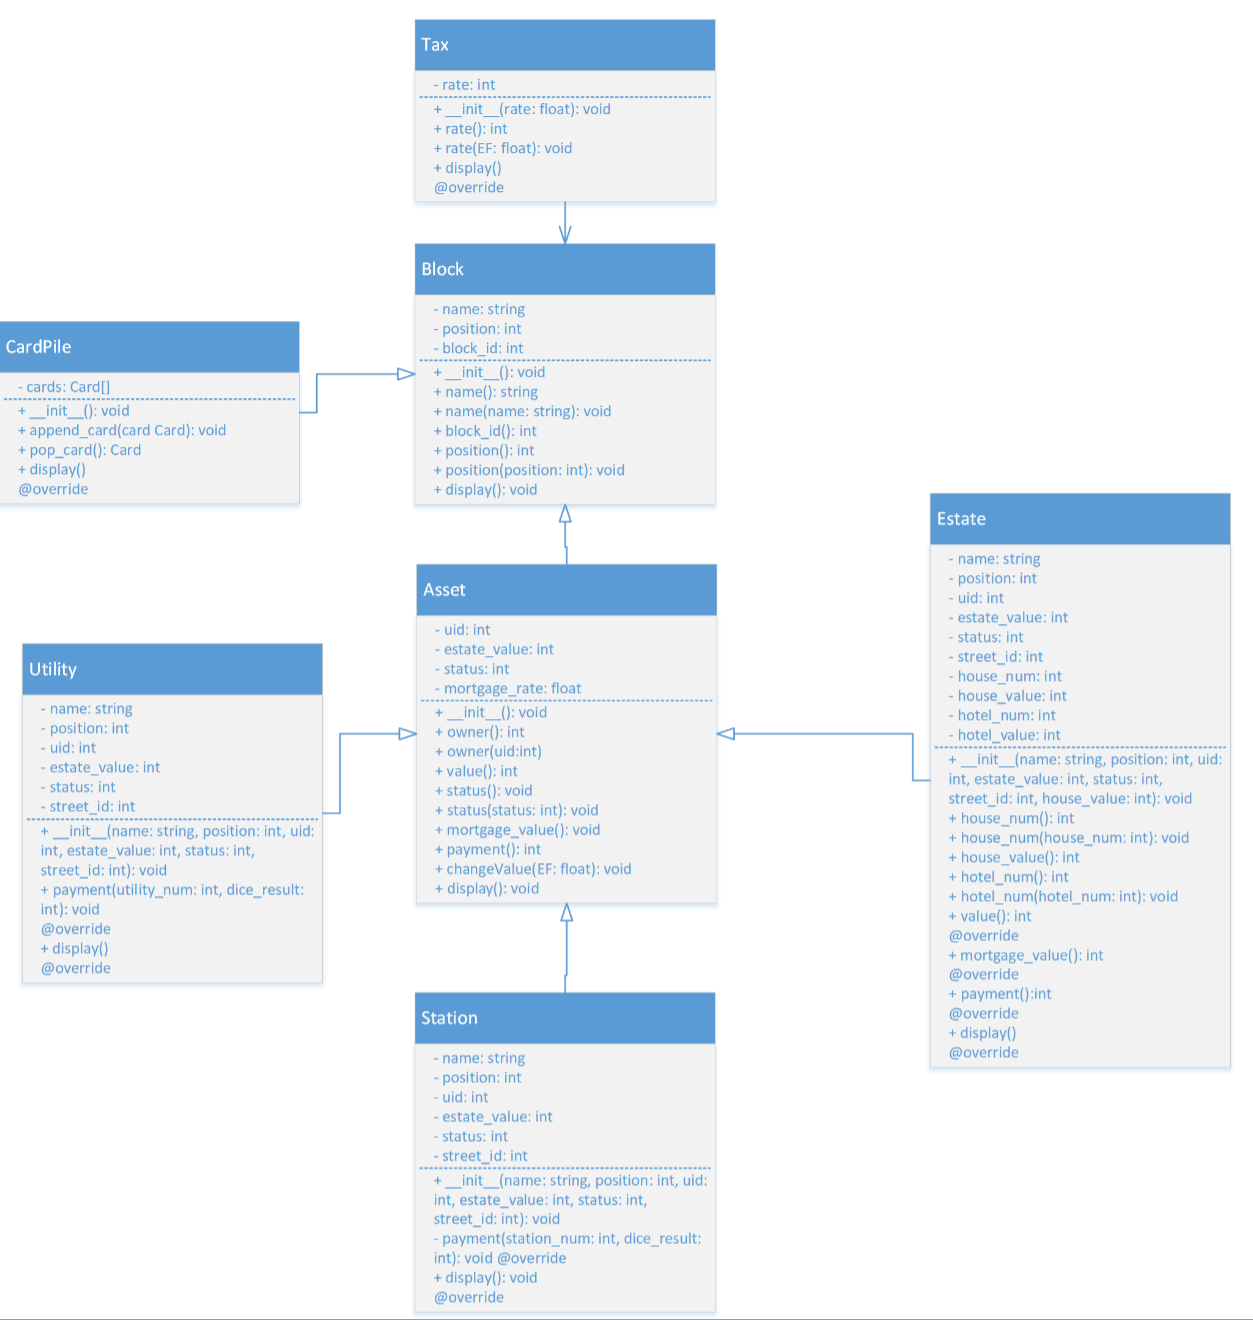
\includegraphics[scale=0.9]{image/Block.png}
\\
\\
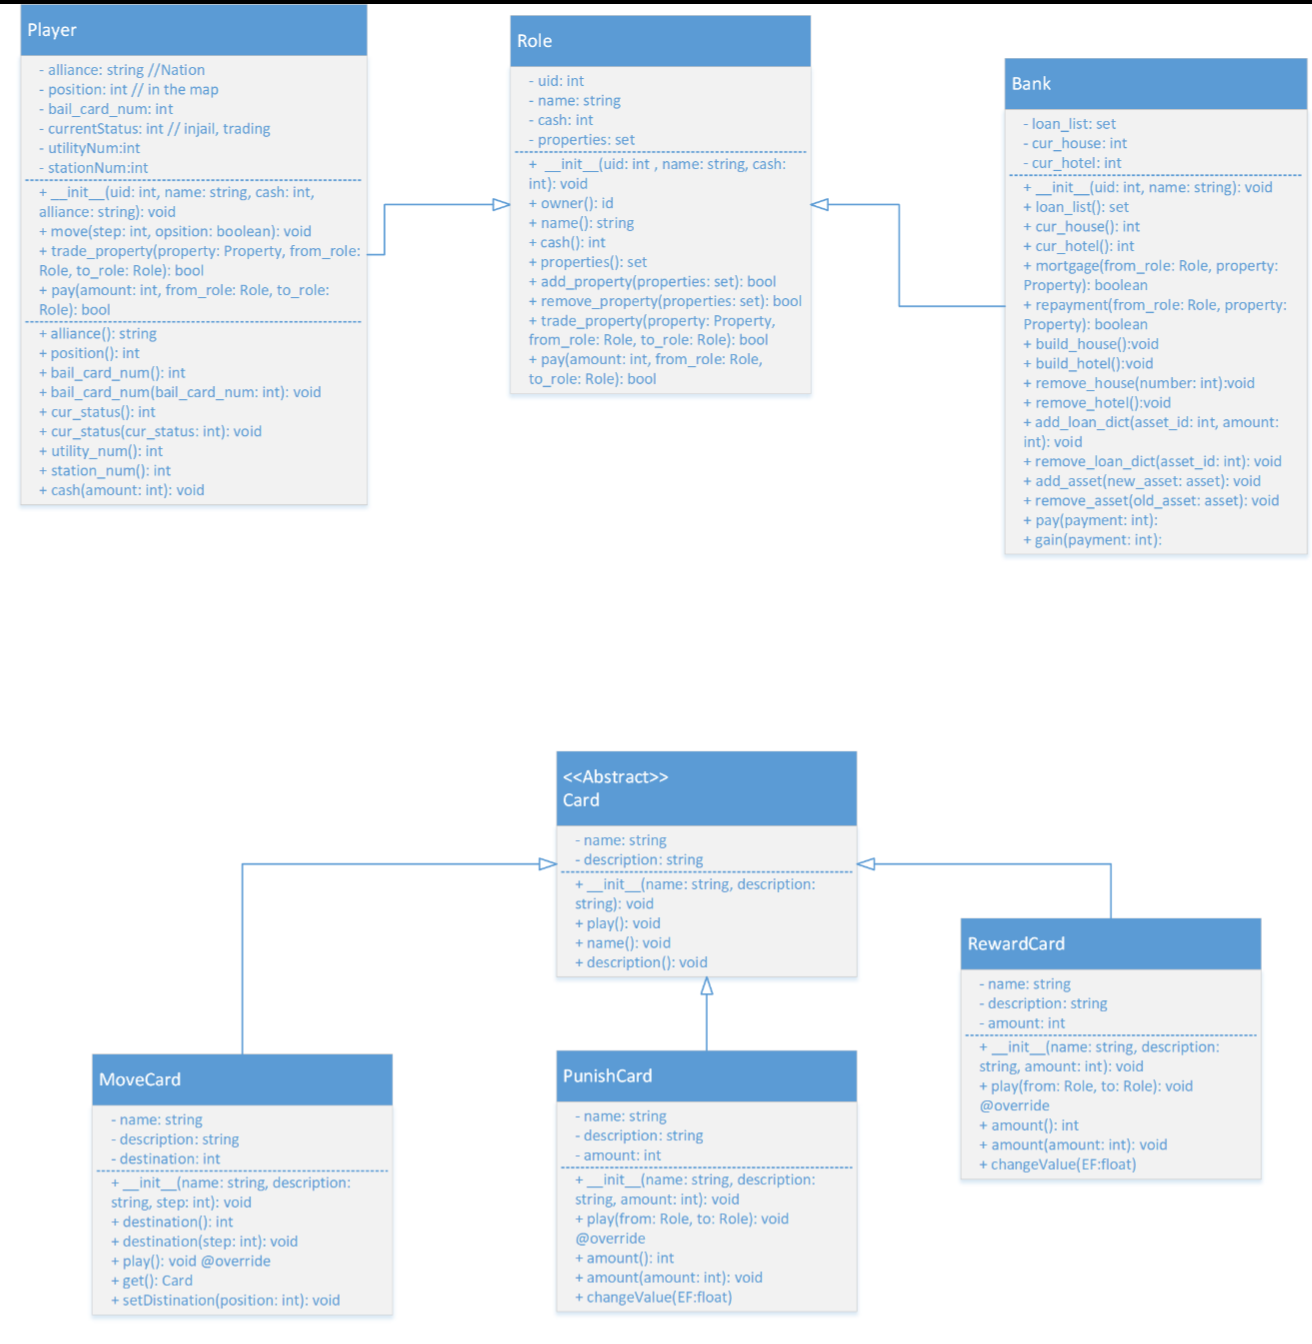
\includegraphics[scale=0.9]{image/roleandcard.png}
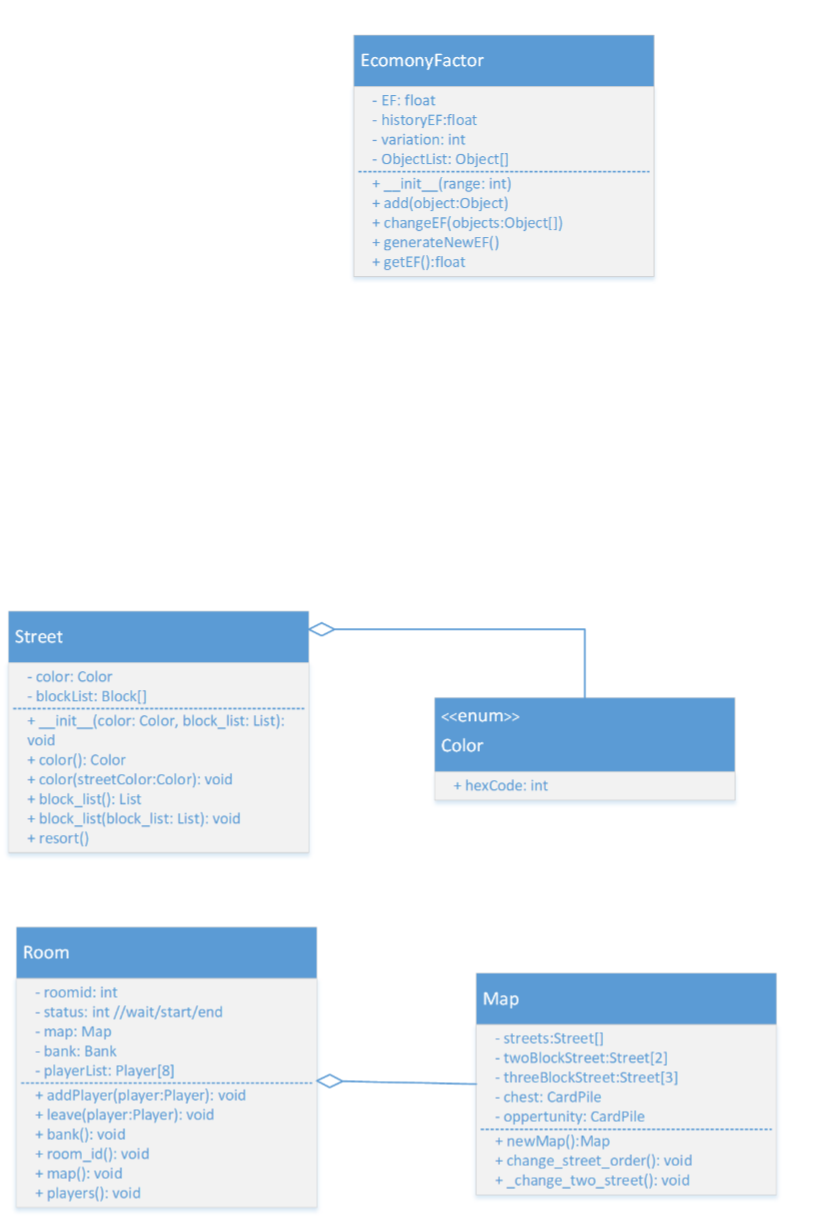
\includegraphics[scale=1.3]{image/efandmain.png}
\section*{Appendix II-UI}
\begin{figure}[htbp]
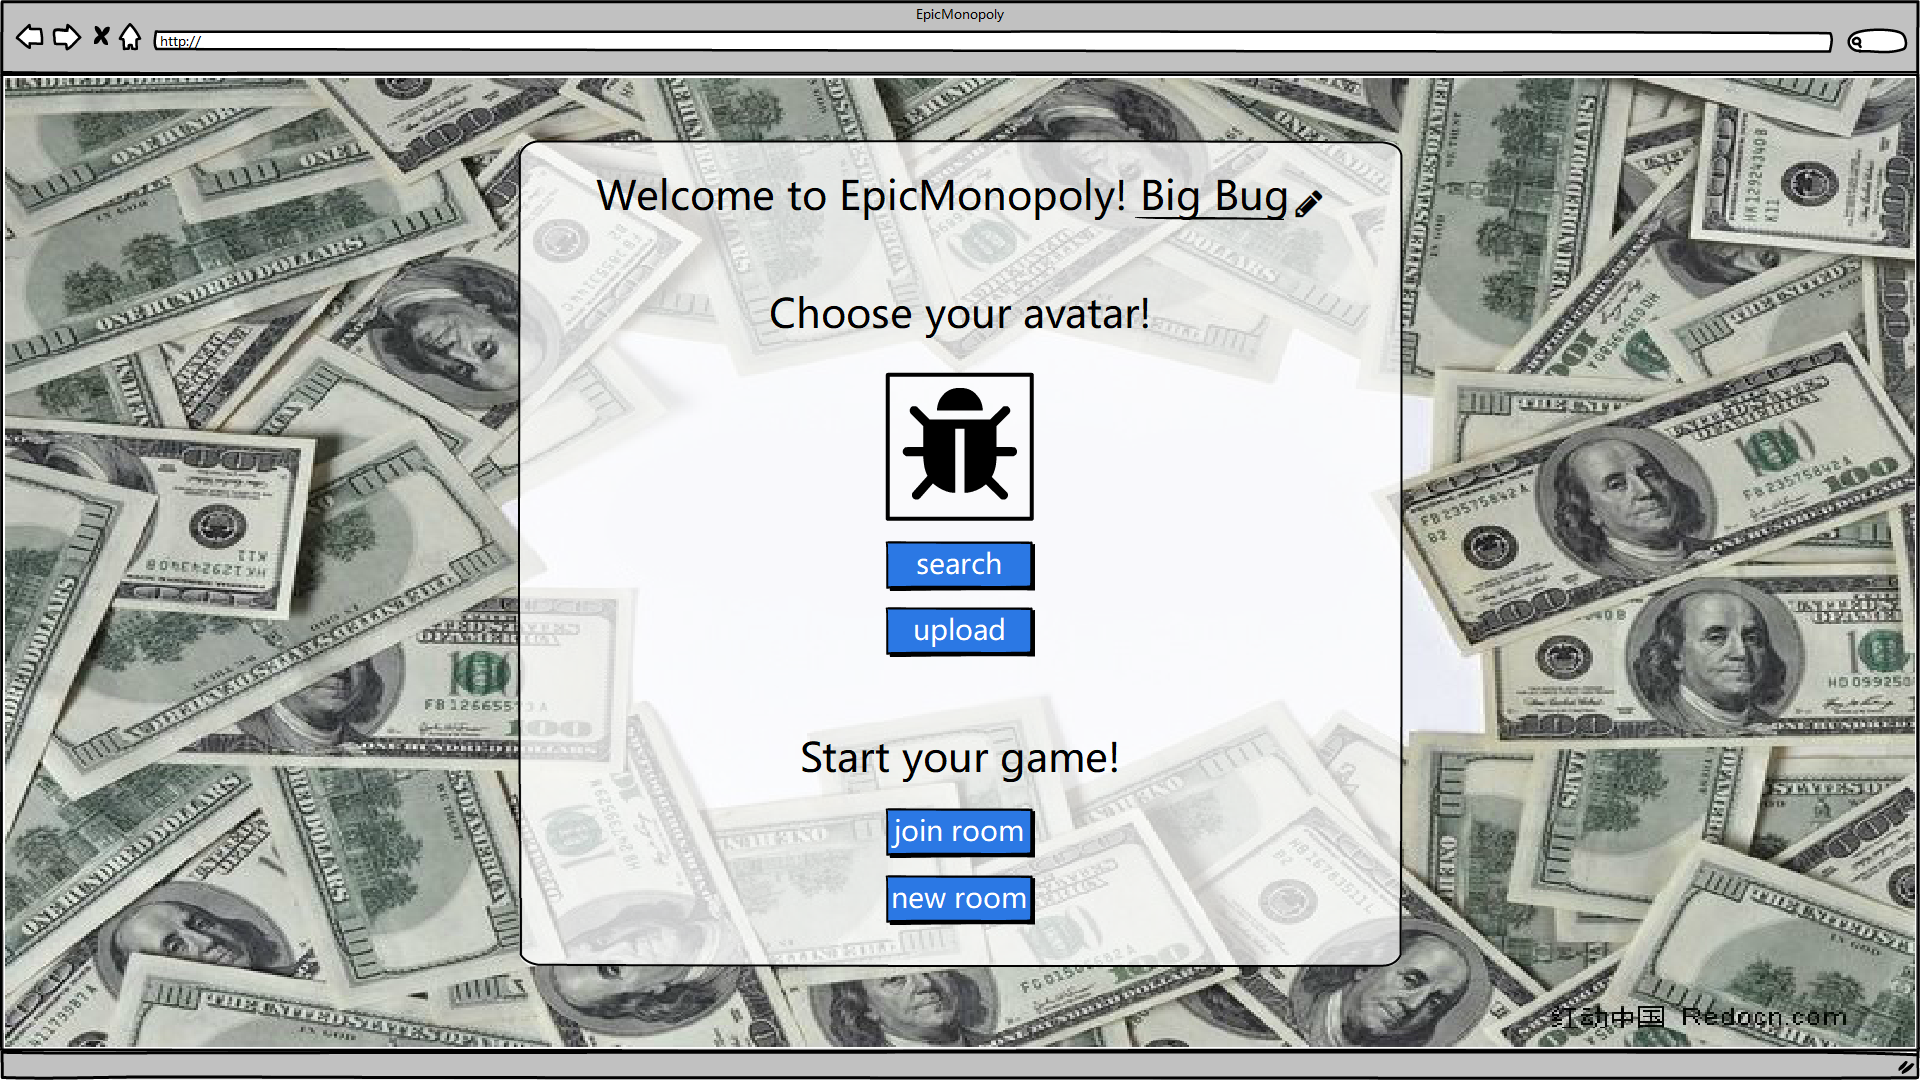
\includegraphics[scale=0.18]{image/pre_game_setting.png}
\caption{Login page}

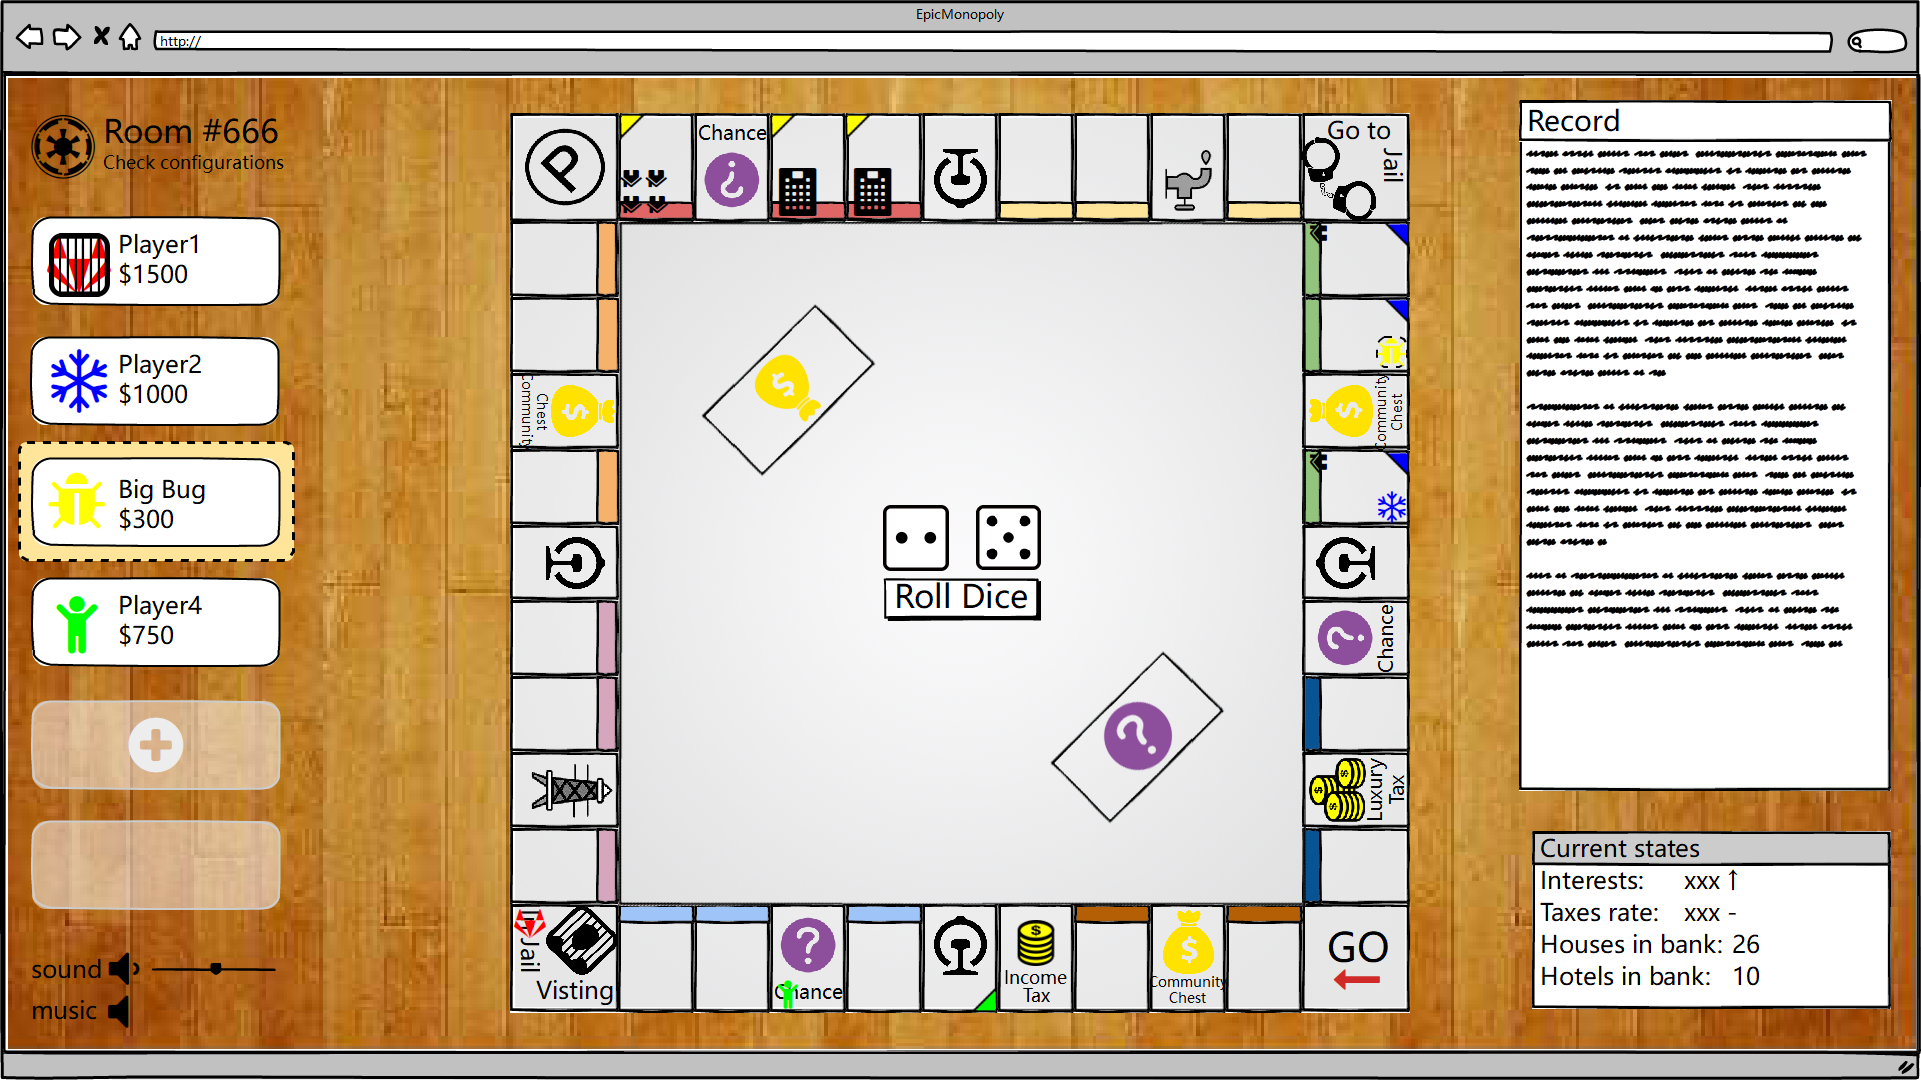
\includegraphics[scale=0.18]{image/in_game_main.png}
\caption{Main page}

\end{figure}
\begin{figure}[htbp]
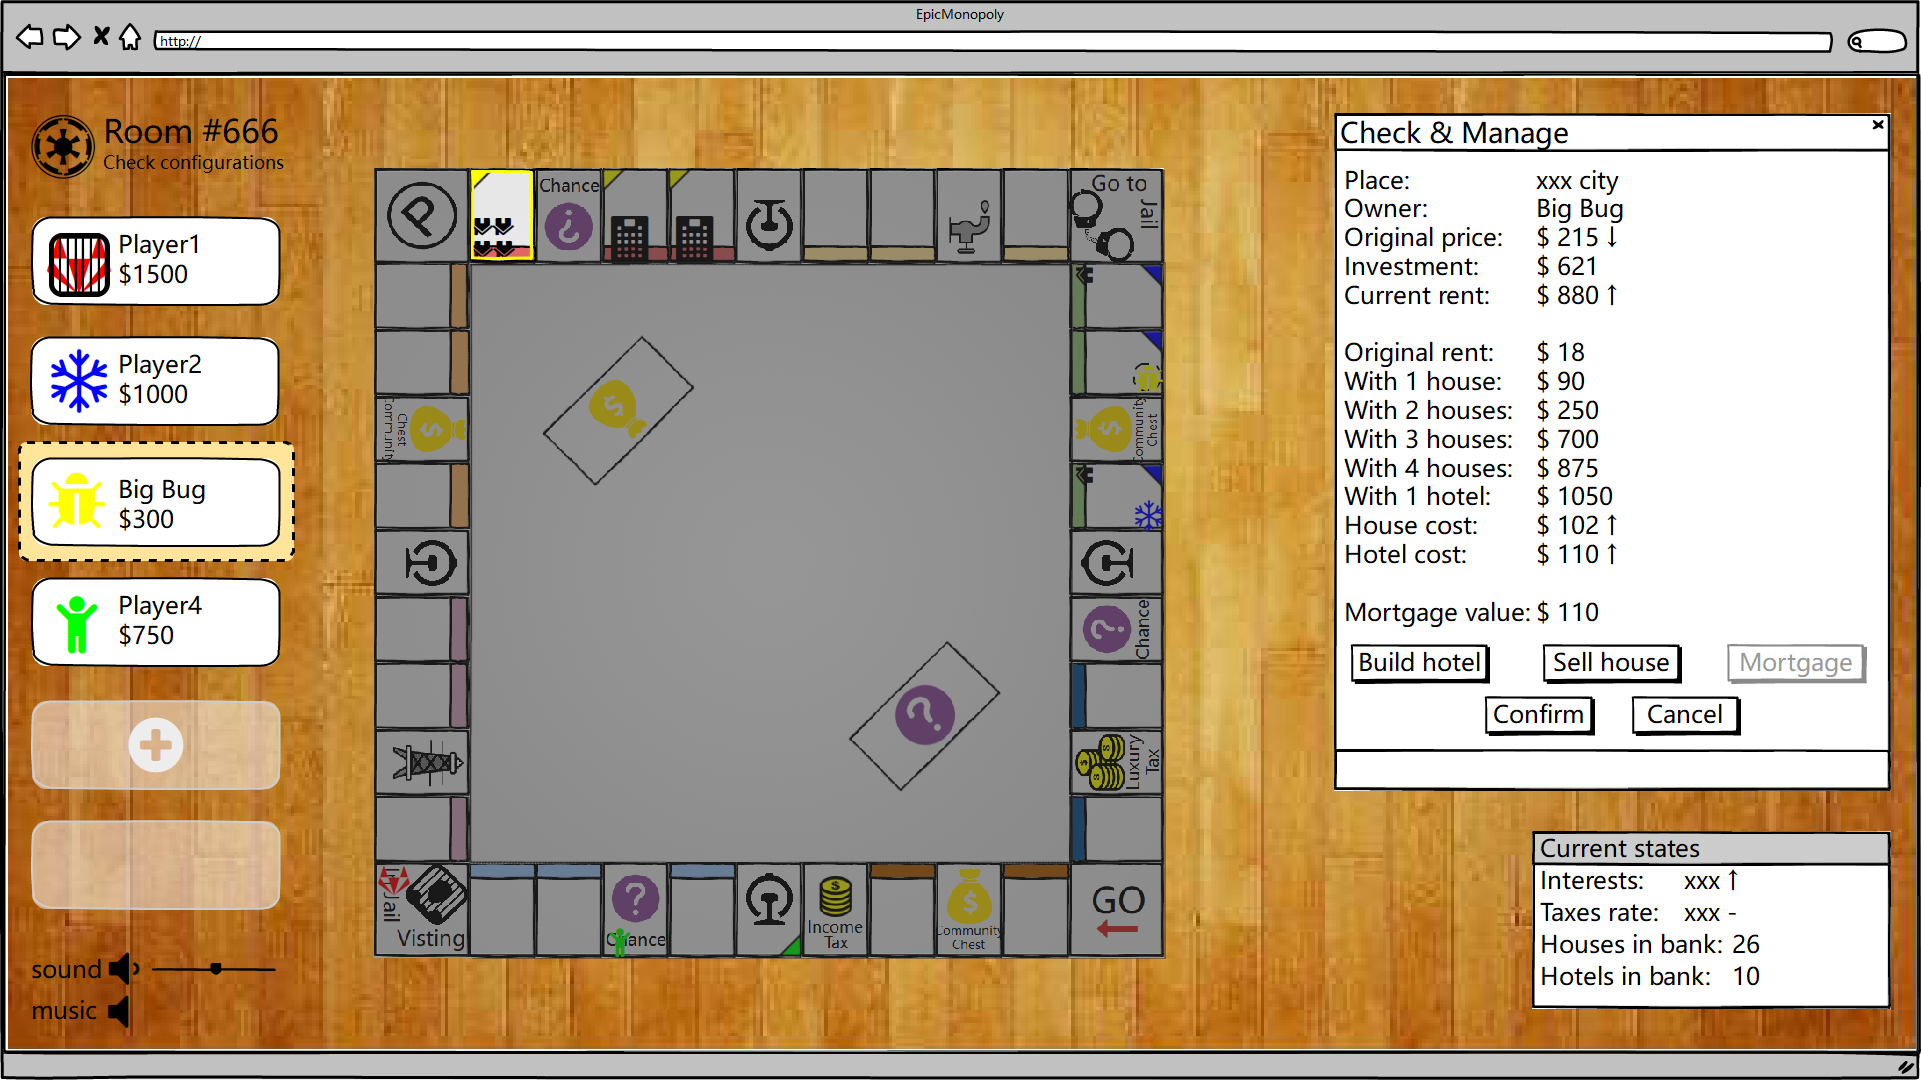
\includegraphics[scale=0.18]{image/in_game_management.png}
\caption{Management page}
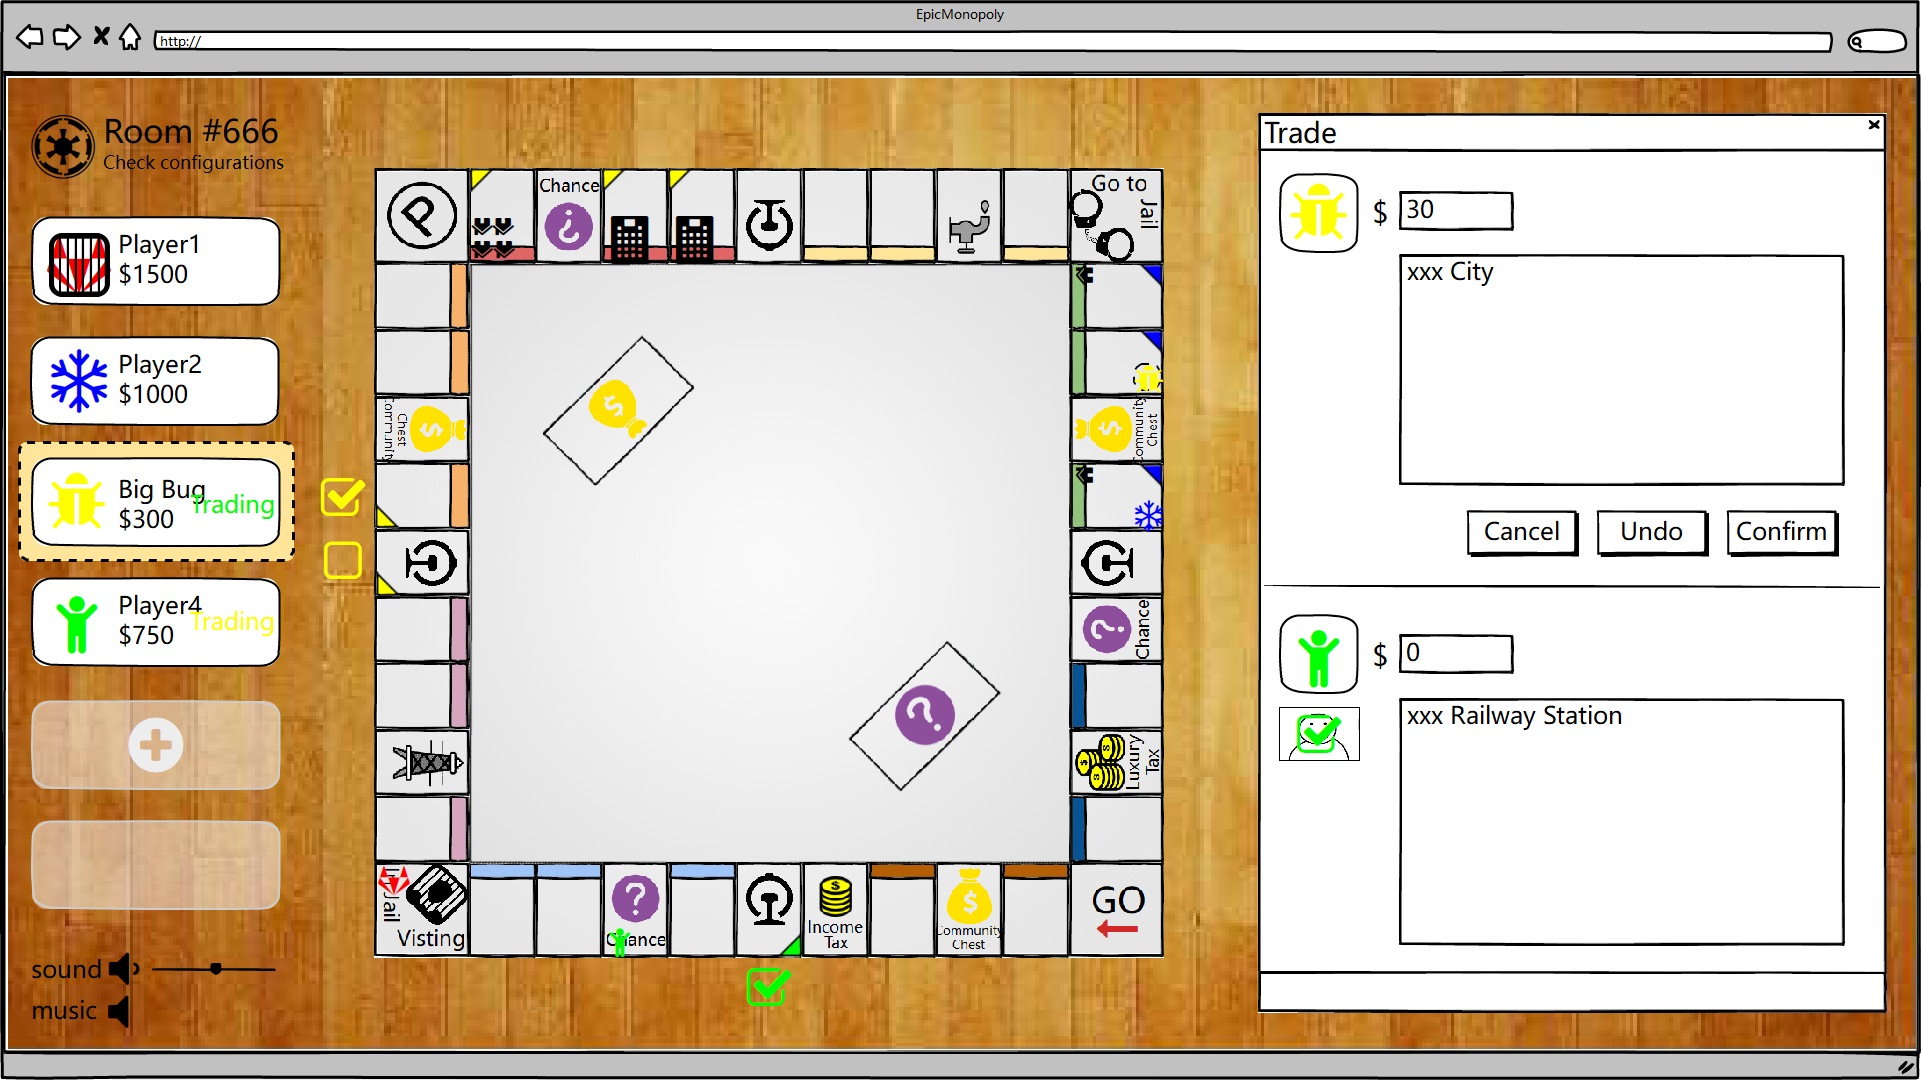
\includegraphics[scale=0.18]{image/in_game_trading.png}
\caption{Trade page}
\end{figure}
\end{document}
